\chapter{Reasonable Title for Main Content}
\label{chap:content}

% Standard structure:
% Formal task description + notation
% Relevant technical background
%% Can refer back to your technical background \Cref{sec:bkg_nerf}.
% Main technical concept
% Architectural details: how the above fits into the network
% Training details

% Words need to go here, two sentences!

% \section{Section heading}
% \label{sec:first_section}

% Also text goes here.

% \subsection{Subsection heading}
% \label{sec:thisone}

% \paragraph{Implementation details. }
% Sentence starts here.

% Replace template text! So many people leave Pascal's words in their final thesis...

% Tables: 
%% See example below
%% tabularx, no vertical lines, toprule, midrule after headings, bottomrule

\begin{table}[!t] % !
\centering
\caption{Ablation study. Meaningful detailed caption full stop. What does the table show? Explain it to me. Who can tell me what a baseline is? Best results are denoted in bold, second-best results are underlined.}
\label{tab:label_here}
\begin{tabularx}{\linewidth}{@{}lCC@{}} % !
\toprule % !
Method & Your Metric $\uparrow$ & Your Other Metric $\downarrow$\\
\midrule % !
Baseline-Random & 3.2 & 12.1 \\
Method A \citep{Oetiker2021LatexIntroduction} & 21.2 & 10.3 \\
Method B \citep{Smith2021Wubalubadubdub} & \underline{21.7} & \textbf{9.8}\\
\midrule % !
Ours & \textbf{22.8} & \underline{9.9}\\
\bottomrule% !
\end{tabularx}
\end{table}

We show in \Cref{tab:label_here} that\dots
Always refer to your tables and figures in the text.

\begin{figure}[!t]
  \includegraphics[width=0.5\linewidth]{figures/escalators.png}
  \caption[Short caption for the index]{A detailed meaningful caption. Longer than you would want in your index.}
  \label{fig:your_label}
\end{figure}%
We show in \Cref{fig:your_label} that\dots

% Subcaption for multiple figures in a grid
An example of a $1\times 2$ subfigure on a $1\times 3$ subfigure is given in \Cref{fig:subfig}. You can also refer to subfigures like \Cref{fig:sub_label_a} or just the sub-label \subref{fig:sub_label_a}. This is also an example of using PGFPlot in your thesis, which builds on top of Tikz (draw with vector graphics within latex).

\begin{figure}[!t]\centering
    \begin{subfigure}[]{0.5\linewidth}\centering % this part takes up 50% of the line
        % qpn_pdf_comparison.tex
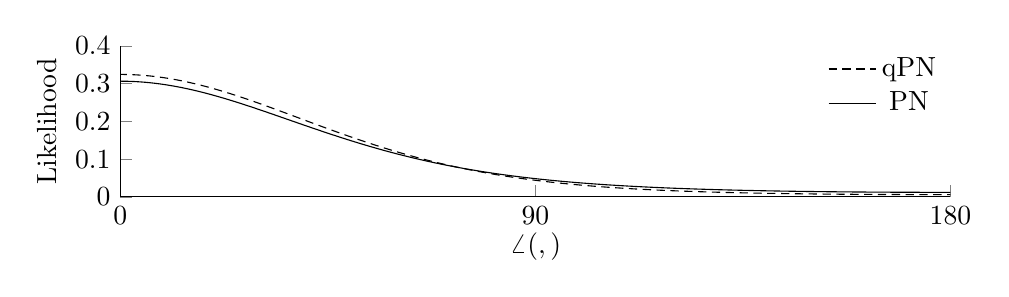
\begin{tikzpicture}
\begin{axis}[
width=\textwidth,
height=3.5cm,
%xmin=-180,
xmin=0,
xmax=180,
xtick={-180, -90, 0, 90, 180},
%xlabel={$\angle(\bbf, \bmu)$ (\textsuperscript{$\circ$})},
xlabel={$\angle(\bbf, \bmu) \vphantom{\rho}$},
xlabel shift=-4pt,
ymin=0,
ymax=0.4,
ytick={0, 0.1,0.2,0.3,0.4},
%ylabel={Relative Likelihood},
ylabel={Likelihood},
%ylabel shift = 1 pt
axis x line*=bottom,
axis y line*=left,
%ymajorticks=false,
%ylabel near ticks,
%hide y axis,
legend entries={qPN,PN},
legend style={draw=none, at={(1,1)}, anchor=north east},
%legend pos=north east,
]

%\addplot [only marks, mark size=2.5pt, mark=*, mark options={solid, black}]
%table[row sep=\\]{
%1 10\\
%};

% vMF for rho = 1
\addplot [black, densely dashed] table [row sep=newline]{
-180	0.00593882225388289
-179.099549774887	0.00594028921694383
-178.199099549775	0.00594469191800688
-177.298649324662	0.00595203579548720
-176.398199099550	0.00596232992266134
-175.497748874437	0.00597558702155373
-174.597298649325	0.00599182348239717
-173.696848424212	0.00601105938868620
-172.796398199100	0.00603331854784825
-171.895947973987	0.00605862852756205
-170.995497748874	0.00608702069775855
-170.095047523762	0.00611853027834409
-169.194597298649	0.00615319639269101
-168.294147073537	0.00619106212694495
-167.393696848424	0.00623217459520314
-166.493246623312	0.00627658501062192
-165.592796398199	0.00632434876251575
-164.692346173087	0.00637552549951384
-163.791895947974	0.00643017921884367
-162.891445722861	0.00648837836181406
-161.990995497749	0.00655019591557253
-161.090545272636	0.00661570952121452
-160.190095047524	0.00668500158832337
-159.289644822411	0.00675815941602121
-158.389194597299	0.00683527532061170
-157.488744372186	0.00691644676989561
-156.588294147074	0.00700177652423943
-155.687843921961	0.00709137278447597
-154.787393696848	0.00718534934671393
-153.886943471736	0.00728382576413018
-152.986493246623	0.00738692751581490
-152.086043021511	0.00749478618273469
-151.185592796398	0.00760753963087304
-150.285142571286	0.00772533220160043
-149.384692346173	0.00784831490931819
-148.484242121061	0.00797664564641068
-147.583791895948	0.00811048939552963
-146.683341670835	0.00825001844922190
-145.782891445723	0.00839541263689825
-144.882441220610	0.00854685955912501
-143.981990995498	0.00870455482920320
-143.081540770385	0.00886870232198060
-142.181090545273	0.00903951442982089
-141.280640320160	0.00921721232563079
-140.380190095048	0.00940202623282070
-139.479739869935	0.00959419570204657
-138.579289644822	0.00979396989455021
-137.678839419710	0.0100016078718829
-136.778389194597	0.0102173788917613
-135.877938969485	0.0104415627097664
-134.977488744372	0.0106744498865556
-134.077038519260	0.0109163421002126
-133.176588294147	0.0111675524633138
-132.276138069035	0.0114284058442382
-131.375687843922	0.0116992391921942
-130.475237618809	0.0119804018653788
-129.574787393697	0.0122722559616246
-128.674337168584	0.0125751766508230
-127.773886943472	0.0128895525083474
-126.873436718359	0.0132157858486230
-125.972986493247	0.0135542930579177
-125.072536268134	0.0139055049253465
-124.172086043022	0.0142698669709984
-123.271635817909	0.0146478397700064
-122.371185592796	0.0150398992712908
-121.470735367684	0.0154465371096080
-120.570285142571	0.0158682609094400
-119.669834917459	0.0163055945791553
-118.769384692346	0.0167590785937651
-117.868934467234	0.0172292702644899
-116.968484242121	0.0177167439932367
-116.068034017009	0.0182220915099724
-115.167583791896	0.0187459220908591
-114.267133566783	0.0192888627548955
-113.366683341671	0.0198515584366881
-112.466233116558	0.0204346721328465
-111.565782891446	0.0210388850193775
-110.665332666333	0.0216648965373200
-109.764882441221	0.0223134244437436
-108.864432216108	0.0229852048251019
-107.963981990996	0.0236809920698135
-107.063531765883	0.0244015587968176
-106.163081540770	0.0251476957367373
-105.262631315658	0.0259202115621660
-104.362181090545	0.0267199326634852
-103.461730865433	0.0275477028665194
-102.561280640320	0.0284043830882373
-101.660830415208	0.0292908509266224
-100.760380190095	0.0302080001807604
-99.8599299649825	0.0311567402971212
-98.9594797398700	0.0321379957379657
-98.0590295147574	0.0331527052677639
-97.1585792896448	0.0342018211534897
-96.2581290645323	0.0352863082746524
-95.3576788394197	0.0364071431389349
-94.4572286143072	0.0375653127993466
-93.5567783891946	0.0387618136688487
-92.6563281640820	0.0399976502284956
-91.7558779389695	0.0412738336252365
-90.8554277138569	0.0425913801556567
-89.9549774887444	0.0439513096320993
-89.0545272636318	0.0453546436278014
-88.1540770385193	0.0468024035979032
-87.2536268134067	0.0482956088734487
-86.3531765882942	0.0498352745257916
-85.4527263631816	0.0514224090991508
-84.5522761380690	0.0530580122094313
-83.6518259129565	0.0547430720078351
-82.7513756878439	0.0564785625082354
-81.8509254627314	0.0582654407777803
-80.9504752376188	0.0601046439907230
-80.0500250125063	0.0619970863460492
-79.1495747873937	0.0639436558500913
-78.2491245622811	0.0659452109659746
-77.3486743371686	0.0680025771324419
-76.4482241120560	0.0701165431553428
-75.5477738869435	0.0722878574758518
-74.6473236618309	0.0745172243202989
-73.7468734367184	0.0768052997373481
-72.8464232116058	0.0791526875291440
-71.9459729864932	0.0815599350839663
-71.0455227613807	0.0840275291188753
-70.1450725362682	0.0865558913417989
-69.2446223111556	0.0891453740434987
-68.3441720860430	0.0917962556308582
-67.4437218609305	0.0945087361139464
-66.5432716358179	0.0972829325603250
-65.6428214107053	0.100118874531089
-64.7423711855928	0.103016499514127
-63.8419209604802	0.105975648371097
-62.9414707353677	0.108996060815557
-62.0410205102551	0.112077370940665
-61.1405702851426	0.115219102815727
-60.2401200600300	0.118420666171763
-59.3396698349175	0.121681352197045
-58.4392196098049	0.125000329464289
-57.5387693846923	0.128376640011893
-56.6383191595798	0.131809195602141
-55.7378689344672	0.135296774179841
-54.8374187093547	0.138838016555232
-53.9369684842421	0.142431423335300
-53.0365182591296	0.146075352127816
-52.1360680340170	0.149768015042453
-51.2356178089045	0.153507476513277
-50.3351675837919	0.157291651466663
-49.4347173586793	0.161118303858358
-48.5342671335668	0.164985045602857
-47.6338169084542	0.168889335917619
-46.7333666833417	0.172828481103815
-45.8329164582291	0.176799634784276
-44.9324662331166	0.180799798618193
-44.0320160080040	0.184825823510745
-43.1315657828915	0.188874411334372
-42.2311155577789	0.192942117176725
-41.3306653326663	0.197025352128509
-40.4302151075538	0.201120386622447
-39.5297648824412	0.205223354332458
-38.6293146573287	0.209330256639849
-37.7288644322161	0.213436967670909
-36.8284142071036	0.217539239907724
-35.9279639819910	0.221632710371378
-35.0275137568784	0.225712907373920
-34.1270635317659	0.229775257832610
-33.2266133066533	0.233815095137021
-32.3261630815408	0.237827667556573
-31.4257128564282	0.241808147173025
-30.5252626313157	0.245751639319396
-29.6248124062031	0.249653192503717
-28.7243621810905	0.253507808792959
-27.8239119559780	0.257310454629482
-26.9234617308654	0.261056072049395
-26.0230115057529	0.264739590269345
-25.1225612806403	0.268355937605495
-24.2221110555278	0.271900053685817
-23.3216608304152	0.275366901914323
-22.4212106053026	0.278751482143549
-21.5207603801901	0.282048843509474
-20.6203101550775	0.285254097381142
-19.7198599299650	0.288362430375528
-18.8194097048524	0.291369117386807
-17.9189594797399	0.294269534577931
-17.0185092546273	0.297059172281551
-16.1180590295148	0.299733647756692
-15.2176088044022	0.302288717747257
-14.3171585792896	0.304720290788432
-13.4167083541771	0.307024439207360
-12.5162581290645	0.309197410765067
-11.6158079039520	0.311235639887556
-10.7153576788394	0.313135758435248
-9.81490745372686	0.314894605961522
-8.91445722861431	0.316509239412957
-8.01400700350175	0.317976942226093
-7.11355677838920	0.319295232777978
-6.21310655327664	0.320461872150507
-5.31265632816408	0.321474871171589
-4.41220610305153	0.322332496699389
-3.51175587793897	0.323033277119411
-2.61130565282641	0.323576007027809
-1.71085542771386	0.323959751078206
-0.810405202601301	0.324183846973289
0.0900450225112556	0.324247907586555
0.990495247623812	0.324151822203856
1.89094547273637	0.323895756878645
2.79139569784892	0.323480153899192
3.69184592296148	0.322905730370374
4.59229614807404	0.322173475916992
5.49274637318659	0.321284649519833
6.39319659829915	0.320240775499918
7.29364682341171	0.319043638670494
8.19409704852426	0.317695278680277
9.09454727363682	0.316197983575280
9.99499749874938	0.314554282610218
10.8954477238619	0.312766938343857
11.7958979489745	0.310838938055944
12.6963481740870	0.308773484526241
13.5967983991996	0.306573986218938
14.4972486243122	0.304244046918075
15.3976988494247	0.301787454861779
16.2981490745373	0.299208171424888
17.1985992996498	0.296510319401079
18.0990495247624	0.293698170936778
18.9994997498749	0.290776135170035
19.8999499749875	0.287748745628064
20.8004002001001	0.284620647437413
21.7008504252126	0.281396584400635
22.6013006503252	0.278081385992965
23.5017508754377	0.274679954331800
24.4022011005503	0.271197251170849
25.3026513256628	0.267638284969552
26.2031015507754	0.264008098086887
27.1035517758879	0.260311754146935
28.0040020010005	0.256554325621615
28.9044522261131	0.252740881673818
29.8049024512256	0.248876476301843
30.7053526763382	0.244966136823481
31.6058029014507	0.241014852735445
32.5062531265633	0.237027564981075
33.4067033516758	0.233009155656326
34.3071535767884	0.228964438181105
35.2076038019010	0.224898147960011
36.1080540270135	0.220814933553444
37.0085042521261	0.216719348377025
37.9089544772386	0.212615842944160
38.8094047023512	0.208508757663596
39.7098549274637	0.204402316200782
40.6103051525763	0.200300619408942
41.5107553776888	0.196207639832926
42.4112056028014	0.192127216786127
43.3116558279140	0.188063051998118
44.2121060530265	0.184018705828143
45.1125562781391	0.179997594037169
46.0130065032516	0.176002985108988
46.9134567283642	0.172037998108720
47.8139069534767	0.168105601065130
48.7143571785893	0.164208609861365
49.6148074037019	0.160349687617115
50.5152576288144	0.156531344543698
51.4157078539270	0.152755938252314
52.3161580790395	0.149025674494559
53.2166083041521	0.145342608313332
54.1170585292646	0.141708645581482
55.0175087543772	0.138125544904884
55.9179589794898	0.134594919866156
56.8184092046023	0.131118241584907
57.7188594297149	0.127696841570189
58.6193096548274	0.124331914840811
59.5197598799400	0.121024523289202
60.4202101050525	0.117775599264758
61.3206603301651	0.114585949352893
62.2211105552777	0.111456258326433
63.1215607803902	0.108387093246516
64.0220110055028	0.105378907690763
64.9224612306153	0.102432046087175
65.8229114557279	0.0995467481329287
66.7233616808404	0.0967231532781166
67.6238119059530	0.0939613052552814
68.5242621310655	0.0912611566365539
69.4247123561781	0.0886225734011217
70.3251625812906	0.0860453394967439
71.2256128064032	0.0835291613800178
72.1260630315158	0.0810736725211163
73.0265132566283	0.0786784378597283
73.9269634817409	0.0763429581999501
74.8274137068534	0.0740666745328909
75.7278639319660	0.0718489722767505
76.6283141570786	0.0696891854251139
77.5287643821911	0.0675866005951714
78.4292146073037	0.0655404609685113
79.3296648324162	0.0635499701180427
80.2301150575288	0.0616142957154864
81.1305652826413	0.0597325731147192
82.0310155077539	0.0579039088070629
82.9314657328664	0.0561273837453856
83.8319159579790	0.0544020565346108
84.7323661830915	0.0527269664869240
85.6328164082041	0.0511011365406147
86.5332666333167	0.0495235760421009
87.4337168584292	0.0479932833912480
88.3341670835418	0.0465092485506194
89.2346173086543	0.0450704554197764
90.1350675337669	0.0436758840761902
91.0355177588794	0.0423245128847245
91.9359679839920	0.0410153204780172
92.8364182091046	0.0397472876104059
93.7368684342171	0.0385193988883359
94.6373186593297	0.0373306443804387
95.5377688844422	0.0361800211106878
96.4382191095548	0.0350665344382275
97.3386693346673	0.0339891993276222
98.2391195597799	0.0329470415134061
99.1395697848924	0.0319390985629079
100.040020010005	0.0309644208414048
100.940470235118	0.0300220723837080
101.840920460230	0.0291111316763113
102.741370685343	0.0282306923542451
103.641820910455	0.0273798638167670
104.542271135568	0.0265577717659938
105.442721360680	0.0257635586725385
106.343171585793	0.0249963841721591
107.243621810905	0.0242554253973593
108.144072036018	0.0235398772478007
109.044522261131	0.0228489526032991
109.944972486243	0.0221818824830783
110.845422711356	0.0215379161548540
111.745872936468	0.0209163211972065
112.646323161581	0.0203163835185896
113.546773386693	0.0197374073362014
114.447223611806	0.0191787151178225
115.347673836918	0.0186396474896023
116.248124062031	0.0181195631126486
117.148574287144	0.0176178385311507
118.049024512256	0.0171338679946382
118.949474737369	0.0166670632568543
119.849924962481	0.0162168533535965
120.750375187594	0.0157826843617553
121.650825412706	0.0153640191416623
122.551275637819	0.0149603370647366
123.451725862931	0.0145711337283091
124.352176088044	0.0141959206593846
125.252626313157	0.0138342250089991
126.153076538269	0.0134855892387171
127.053526763382	0.0131495708007177
127.953976988494	0.0128257418128139
128.854427213607	0.0125136887296590
129.754877438719	0.0122130120113005
130.655327663832	0.0119233257901550
131.555777888944	0.0116442575373965
132.456228114057	0.0113754477296674
133.356678339170	0.0111165495169503
134.257128564282	0.0108672283923641
135.157578789395	0.0106271618645816
136.058029014507	0.0103960391335011
136.958479239620	0.0101735607697450
137.858929464732	0.00995943839850056
138.759379689845	0.00975339438816534
139.659829914958	0.00955516154420918
140.560280140070	0.00936448280861884
141.460730365183	0.00918111096524667
142.361180590295	0.00900480835134479
143.261630815408	0.00883534657552832
144.162081040520	0.00867250624237614
145.062531265633	0.00851607668384570
145.962981490745	0.00836585569764833
146.863431715858	0.00822164929270443
147.763881940971	0.00808327144177255
148.664332166083	0.00795054384132413
149.564782391196	0.00782329567871407
150.465232616308	0.00770136340667929
151.365682841421	0.00758459052517991
152.266133066533	0.00747282737058265
153.166583291646	0.00736593091217264
154.067033516758	0.00726376455596731
154.967483741871	0.00716619795579612
155.867933966984	0.00707310683159993
156.768384192096	0.00698437279489645
157.668834417209	0.00689988318135106
158.569284642321	0.00681953089038679
159.469734867434	0.00674321423176262
160.370185092546	0.00667083677904544
161.270635317659	0.00660230722989844
162.171085542771	0.00653753927310657
163.071535767884	0.00647645146225863
163.971985992996	0.00641896709600501
164.872436218109	0.00636501410481030
165.772886443222	0.00631452494412067
166.673336668334	0.00626743649386745
167.573786893447	0.00622368996423001
168.474237118559	0.00618323080758322
169.374687343672	0.00614600863655781
170.275137568784	0.00611197714814487
171.175587793897	0.00608109405377900
172.076038019010	0.00605332101533875
172.976488244122	0.00602862358700687
173.876938469235	0.00600697116293698
174.777388694347	0.00598833693067831
175.677838919460	0.00597269783031428
176.578289144572	0.00596003451927622
177.478739369685	0.00595033134279801
178.379189594797	0.00594357630998300
179.279639819910	0.00593976107545976
180	0.00593882225388289
};

%% PN
\addplot [black] table [row sep=newline]{
-180	0.0119906989306336
-179.099549774887	0.0119924933487507
-178.199099549775	0.0119978781223270
-177.298649324662	0.0120068578108691
-176.398199099550	0.0120194400196602
-175.497748874437	0.0120356354089268
-174.597298649325	0.0120554577066834
-173.696848424212	0.0120789237252725
-172.796398199100	0.0121060533816135
-171.895947973987	0.0121368697211852
-170.995497748874	0.0121713989457638
-170.095047523762	0.0122096704449472
-169.194597298649	0.0122517168314967
-168.294147073537	0.0122975739805326
-167.393696848424	0.0123472810726244
-166.493246623312	0.0124008806408154
-165.592796398199	0.0124584186216331
-164.692346173087	0.0125199444101309
-163.791895947974	0.0125855109190170
-162.891445722861	0.0126551746419258
-161.990995497749	0.0127289957208917
-161.090545272636	0.0128070380180870
-160.190095047524	0.0128893691918895
-159.289644822411	0.0129760607773467
-158.389194597299	0.0130671882711076
-157.488744372186	0.0131628312208932
-156.588294147074	0.0132630733195801
-155.687843921961	0.0133680025039734
-154.787393696848	0.0134777110583450
-153.886943471736	0.0135922957228169
-152.986493246623	0.0137118578066671
-152.086043021511	0.0138365033066380
-151.185592796398	0.0139663430303262
-150.285142571286	0.0141014927247333
-149.384692346173	0.0142420732100540
-148.484242121061	0.0143882105187790
-147.583791895948	0.0145400360401849
-146.683341670835	0.0146976866702847
-145.782891445723	0.0148613049673048
-144.882441220610	0.0150310393127519
-143.981990995498	0.0152070440781300
-143.081540770385	0.0153894797973578
-142.181090545273	0.0155785133449334
-141.280640320160	0.0157743181198836
-140.380190095048	0.0159770742355263
-139.479739869935	0.0161869687150638
-138.579289644822	0.0164041956930150
-137.678839419710	0.0166289566224783
-136.778389194597	0.0168614604882065
-135.877938969485	0.0171019240254559
-134.977488744372	0.0173505719445543
-134.077038519260	0.0176076371611163
-133.176588294147	0.0178733610318069
-132.276138069035	0.0181479935955373
-131.375687843922	0.0184317938199456
-130.475237618809	0.0187250298529901
-129.574787393697	0.0190279792794509
-128.674337168584	0.0193409293821035
-127.773886943472	0.0196641774072886
-126.873436718359	0.0199980308345694
-125.972986493247	0.0203428076501180
-125.072536268134	0.0206988366234338
-124.172086043022	0.0210664575869432
-123.271635817909	0.0214460217179814
-122.371185592796	0.0218378918225958
-121.470735367684	0.0222424426205569
-120.570285142571	0.0226600610308921
-119.669834917459	0.0230911464571939
-118.769384692346	0.0235361110718786
-117.868934467234	0.0239953800984951
-116.968484242121	0.0244693920911020
-116.068034017009	0.0249585992096429
-115.167583791896	0.0254634674901583
-114.267133566783	0.0259844771085773
-113.366683341671	0.0265221226367289
-112.466233116558	0.0270769132891049
-111.565782891446	0.0276493731587966
-110.665332666333	0.0282400414409081
-109.764882441221	0.0288494726416270
-108.864432216108	0.0294782367710057
-107.963981990996	0.0301269195173747
-107.063531765883	0.0307961224011693
-106.163081540770	0.0314864629058132
-105.262631315658	0.0321985745831513
-104.362181090545	0.0329331071307785
-103.461730865433	0.0336907264384522
-102.561280640320	0.0344721146006246
-101.660830415208	0.0352779698919657
-100.760380190095	0.0361090067025907
-99.8599299649825	0.0369659554295389
-98.9594797398700	0.0378495623208916
-98.0590295147574	0.0387605892687499
-97.1585792896448	0.0396998135471348
-96.2581290645323	0.0406680274907127
-95.3576788394197	0.0416660381100942
-94.4572286143072	0.0426946666393070
-93.5567783891946	0.0437547480108987
-92.6563281640820	0.0448471302539957
-91.7558779389695	0.0459726738105186
-90.8554277138569	0.0471322507646448
-89.9549774887444	0.0483267439805150
-89.0545272636318	0.0495570461430989
-88.1540770385193	0.0508240586970770
-87.2536268134067	0.0521286906785591
-86.3531765882942	0.0534718574344416
-85.4527263631816	0.0548544792242272
-84.5522761380690	0.0562774796991667
-83.6518259129565	0.0577417842536665
-82.7513756878439	0.0592483182440138
-81.8509254627314	0.0607980050696284
-80.9504752376188	0.0623917641122447
-80.0500250125063	0.0640305085286670
-79.1495747873937	0.0657151428930373
-78.2491245622811	0.0674465606848951
-77.3486743371686	0.0692256416197082
-76.4482241120560	0.0710532488190156
-75.5477738869435	0.0729302258178402
-74.6473236618309	0.0748573934076153
-73.7468734367184	0.0768355463135238
-72.8464232116058	0.0788654497058654
-71.9459729864932	0.0809478355458653
-71.0455227613807	0.0830833987672009
-70.1450725362682	0.0852727932954634
-69.2446223111556	0.0875166279087852
-68.3441720860430	0.0898154619439534
-67.4437218609305	0.0921698008534908
-66.5432716358179	0.0945800916204203
-65.6428214107053	0.0970467180387348
-64.7423711855928	0.0995699958689617
-63.8419209604802	0.102150167879651
-62.9414707353677	0.104787398787101
-62.0410205102551	0.107481770107189
-61.1405702851426	0.110233274934753
-60.2401200600300	0.113041812667600
-59.3396698349175	0.115907183693877
-58.4392196098049	0.118829084063194
-57.5387693846923	0.121807100163588
-56.6383191595798	0.124840703428048
-55.7378689344672	0.127929245096019
-54.8374187093547	0.131071951056859
-53.9369684842421	0.134267916803817
-53.0365182591296	0.137516102528583
-52.1360680340170	0.140815328387842
-51.2356178089045	0.144164269974586
-50.3351675837919	0.147561454028085
-49.4347173586793	0.151005254417467
-48.5342671335668	0.154493888434676
-47.6338169084542	0.158025413433309
-46.7333666833417	0.161597723850231
-45.8329164582291	0.165208548647185
-44.9324662331166	0.168855449209545
-44.0320160080040	0.172535817739138
-43.1315657828915	0.176246876177505
-42.2311155577789	0.179985675695130
-41.3306653326663	0.183749096781007
-40.4302151075538	0.187533849965474
-39.5297648824412	0.191336477207404
-38.6293146573287	0.195153353974725
-37.7288644322161	0.198980692044767
-36.8284142071036	0.202814543048072
-35.9279639819910	0.206650802776185
-35.0275137568784	0.210485216270395
-34.1270635317659	0.214313383704607
-33.2266133066533	0.218130767071368
-32.3261630815408	0.221932697675633
-31.4257128564282	0.225714384436182
-30.5252626313157	0.229470922989612
-29.6248124062031	0.233197305586701
-28.7243621810905	0.236888431765564
-27.8239119559780	0.240539119780551
-26.9234617308654	0.244144118760249
-26.0230115057529	0.247698121562262
-25.1225612806403	0.251195778286845
-24.2221110555278	0.254631710405784
-23.3216608304152	0.258000525457425
-22.4212106053026	0.261296832253363
-21.5207603801901	0.264515256537099
-20.6203101550775	0.267650457030071
-19.7198599299650	0.270697141795823
-18.8194097048524	0.273650084848816
-17.9189594797399	0.276504142930569
-17.0185092546273	0.279254272372396
-16.1180590295148	0.281895545961159
-15.2176088044022	0.284423169722143
-14.3171585792896	0.286832499531416
-13.4167083541771	0.289119057468932
-12.5162581290645	0.291278547823218
-11.6158079039520	0.293306872658652
-10.7153576788394	0.295200146857297
-9.81490745372686	0.296954712548851
-8.91445722861431	0.298567152844551
-8.01400700350175	0.300034304793906
-7.11355677838920	0.301353271486775
-6.21310655327664	0.302521433227634
-5.31265632816408	0.303536457713867
-4.41220610305153	0.304396309155400
-3.51175587793897	0.305099256279153
-2.61130565282641	0.305643879168329
-1.71085542771386	0.306029074893636
-0.810405202601301	0.306254061900917
0.0900450225112556	0.306318383127454
0.990495247623812	0.306221907827150
1.89094547273637	0.305964832093011
2.79139569784892	0.305547678073595
3.69184592296148	0.304971291888406
4.59229614807404	0.304236840255493
5.49274637318659	0.303345805852625
6.39319659829915	0.302299981441372
7.29364682341171	0.301101462791123
8.19409704852426	0.299752640447376
9.09454727363682	0.298256190395652
9.99499749874938	0.296615063678810
10.8954477238619	0.294832475031592
11.7958979489745	0.292911890601618
12.6963481740870	0.290857014830893
13.5967983991996	0.288671776576093
14.4972486243122	0.286360314549431
15.3976988494247	0.283926962164750
16.2981490745373	0.281376231875679
17.1985992996498	0.278712799094137
18.0990495247624	0.275941485778241
18.9994997498749	0.273067243778772
19.8999499749875	0.270095138032765
20.8004002001001	0.267030329691546
21.7008504252126	0.263878059268716
22.6013006503252	0.260643629891121
23.5017508754377	0.257332390732894
24.4022011005503	0.253949720709172
25.3026513256628	0.250501012502138
26.2031015507754	0.246991656987747
27.1035517758879	0.243427028126757
28.0040020010005	0.239812468378738
28.9044522261131	0.236153274692489
29.8049024512256	0.232454685120866
30.7053526763382	0.228721866102504
31.6058029014507	0.224959900447232
32.5062531265633	0.221173776056372
33.4067033516758	0.217368375403432
34.3071535767884	0.213548465795149
35.2076038019010	0.209718690427359
36.1080540270135	0.205883560244867
37.0085042521261	0.202047446609377
37.9089544772386	0.198214574774610
38.8094047023512	0.194389018163117
39.7098549274637	0.190574693434904
40.6103051525763	0.186775356333922
41.5107553776888	0.182994598294684
42.4112056028014	0.179235843787884
43.3116558279140	0.175502348380736
44.2121060530265	0.171797197485050
45.1125562781391	0.168123305763601
46.0130065032516	0.164483417163314
46.9134567283642	0.160880105542022
47.8139069534767	0.157315775854166
48.7143571785893	0.153792665859714
49.6148074037019	0.150312848319809
50.5152576288144	0.146878233642130
51.4157078539270	0.143490572938805
52.3161580790395	0.140151461459694
53.2166083041521	0.136862342364202
54.1170585292646	0.133624510795262
55.0175087543772	0.130439118219859
55.9179589794898	0.127307177001348
56.8184092046023	0.124229565169881
57.7188594297149	0.121207031358439
58.6193096548274	0.118240199873322
59.5197598799400	0.115329575869312
60.4202101050525	0.112475550601280
61.3206603301651	0.109678406725546
62.2211105552777	0.106938323625934
63.1215607803902	0.104255382741110
64.0220110055028	0.101629572871462
64.9224612306153	0.0990607954454620
65.8229114557279	0.0965488697271070
66.7233616808404	0.0940935379476967
67.6238119059530	0.0916944703468125
68.5242621310655	0.0893512701089511
69.4247123561781	0.0870634781837980
70.3251625812906	0.0848305779796060
71.2256128064032	0.0826519999205657
72.1260630315158	0.0805271258604151
73.0265132566283	0.0784552933458236
73.9269634817409	0.0764357997243074
74.8274137068534	0.0744679060925798
75.7278639319660	0.0725508410823142
76.6283141570786	0.0706838044812976
77.5287643821911	0.0688659706888748
78.4292146073037	0.0670964920054378
79.3296648324162	0.0653745017564913
80.2301150575288	0.0636991172525342
81.1305652826413	0.0620694425866342
82.0310155077539	0.0604845712721466
82.9314657328664	0.0589435887235342
83.8319159579790	0.0574455745836922
84.7323661830915	0.0559896049015723
85.6328164082041	0.0545747541642304
86.5332666333167	0.0532000971877051
87.4337168584292	0.0518647108713675
88.3341670835418	0.0505676758205666
89.2346173086543	0.0493080778425443
90.1350675337669	0.0480850093206959
91.0355177588794	0.0468975704723242
91.9359679839920	0.0457448704950738
92.8364182091046	0.0446260286072388
93.7368684342171	0.0435401749871184
94.6373186593297	0.0424864516165557
95.5377688844422	0.0414640130337261
96.4382191095548	0.0404720270001645
97.3386693346673	0.0395096750869173
98.2391195597799	0.0385761531845954
99.1395697848924	0.0376706719419775
100.040020010005	0.0367924571376785
100.940470235118	0.0359407499892537
101.840920460230	0.0351148074039608
102.741370685343	0.0343139021752434
103.641820910455	0.0335373231288448
104.542271135568	0.0327843752222949
105.442721360680	0.0320543796013528
106.343171585793	0.0313466736168243
107.243621810905	0.0306606108050087
108.144072036018	0.0299955608348703
109.044522261131	0.0293509094248696
109.944972486243	0.0287260582322320
110.845422711356	0.0281204247172808
111.745872936468	0.0275334419853084
112.646323161581	0.0269645586083166
113.546773386693	0.0264132384288159
114.447223611806	0.0258789603477341
115.347673836918	0.0253612180983568
116.248124062031	0.0248595200080942
117.148574287144	0.0243733887497451
118.049024512256	0.0239023610838160
118.949474737369	0.0234459875933402
119.849924962481	0.0230038324125352
120.750375187594	0.0225754729505372
121.650825412706	0.0221604996113556
122.551275637819	0.0217585155110976
123.451725862931	0.0213691361934304
124.352176088044	0.0209919893441646
125.252626313157	0.0206267145057666
126.153076538269	0.0202729627925378
127.053526763382	0.0199303966071268
127.953976988494	0.0195986893589825
128.854427213607	0.0192775251852916
129.754877438719	0.0189665986748924
130.655327663832	0.0186656145956038
131.555777888944	0.0183742876253586
132.456228114057	0.0180923420874891
133.356678339170	0.0178195116904673
134.257128564282	0.0175555392723672
135.157578789395	0.0173001765502783
136.058029014507	0.0170531838748695
136.958479239620	0.0168143299902687
137.858929464732	0.0165833917994001
138.759379689845	0.0163601541348916
139.659829914958	0.0161444095356449
140.560280140070	0.0159359580291380
141.460730365183	0.0157346069195101
142.361180590295	0.0155401705814634
143.261630815408	0.0153524702599989
144.162081040520	0.0151713338759902
145.062531265633	0.0149965958375855
145.962981490745	0.0148280968574177
146.863431715858	0.0146656837755925
147.763881940971	0.0145092093884149
148.664332166083	0.0143585322828070
149.564782391196	0.0142135166763634
150.465232616308	0.0140740322629848
151.365682841421	0.0139399540640257
152.266133066533	0.0138111622848871
153.166583291646	0.0136875421769826
154.067033516758	0.0135689839050041
154.967483741871	0.0134553824194098
155.867933966984	0.0133466373340562
156.768384192096	0.0132426528088973
157.668834417209	0.0131433374376688
158.569284642321	0.0130486041404809
159.469734867434	0.0129583700612387
160.370185092546	0.0128725564698137
161.270635317659	0.0127910886688885
162.171085542771	0.0127138959054001
163.071535767884	0.0126409112865073
163.971985992996	0.0125720717000112
164.872436218109	0.0125073177391591
165.772886443222	0.0124465936317643
166.673336668334	0.0123898471735780
167.573786893447	0.0123370296658506
168.474237118559	0.0122880958570252
169.374687343672	0.0122430038885056
170.275137568784	0.0122017152444478
171.175587793897	0.0121641947055252
172.076038019010	0.0121304103066208
172.976488244122	0.0121003332984059
173.876938469235	0.0120739381127641
174.777388694347	0.0120512023320271
175.677838919460	0.0120321066619893
176.578289144572	0.0120166349086751
177.478739369685	0.0120047739588320
178.379189594797	0.0119965137641322
179.279639819910	0.0119918473290633
180	0.0119906989306336
};

\end{axis}
\end{tikzpicture}
        \vspace{-18pt}
        \caption{Relative likelihood ($\rho = 1$)}
        \label{fig:sub_label_a}
    \end{subfigure}\hfill % any excess horizontal space goes between the subfigures
    \begin{subfigure}[]{0.5\linewidth}\centering
        \begin{tikzpicture}
\begin{axis}[
scaled ticks=false,
tick label style={/pgf/number format/fixed},
width=\textwidth,
height=3.5cm,
xmin=0,
xmax=5,
xtick={0, 1, ..., 5},
xlabel={$\rho \vphantom{\angle(\bbf, \bmu)}$},
xlabel shift=-4pt,
ymin=0,
ymax=0.04,
ytick={0, 0.01, ...,0.04},
ylabel={MAE},
%ylabel shift=-2pt,
axis x line*=bottom,
axis y line*=left,
%ymajorticks=false,
%ylabel near ticks,
%hide y axis,
%legend entries={$\vMF$,$\PN$},
%legend style={draw=none, at={(1,1)}, anchor=north east},
%legend pos=north east,
]

%\addplot [only marks, mark size=2.5pt, mark=*, mark options={solid, black}]
%table[row sep=\\]{
%1 10\\
%};

%% MAE
\addplot [black] table [row sep=newline]{
0.100000000000000	0.0413191281236007
0.200000000000000	0.0346139984696496
0.300000000000000	0.0287655282865310
0.400000000000000	0.0237540068813730
0.500000000000000	0.0195422603081568
0.600000000000000	0.0160829910864740
0.700000000000000	0.0133195988920811
0.800000000000000	0.0111819311945709
0.900000000000000	0.00959030244918633
1	0.00845004251628531
1.10000000000000	0.00766221054548387
1.20000000000000	0.00713263091784733
1.30000000000000	0.00678074719239092
1.40000000000000	0.00654514421515479
1.50000000000000	0.00637890241051719
1.60000000000000	0.00625222568688656
1.70000000000000	0.00614385236628324
1.80000000000000	0.00604225040266751
1.90000000000000	0.00594325703404724
2	0.00584243421372227
2.10000000000000	0.00573946498348980
2.20000000000000	0.00563494957933974
2.30000000000000	0.00552965882016238
2.40000000000000	0.00542408740054571
2.50000000000000	0.00531819228966805
2.60000000000000	0.00521173034184175
2.70000000000000	0.00510893640257420
2.80000000000000	0.00500440880697224
2.90000000000000	0.00490423025006244
3.00000000000000	0.00480464961892366
3.10000000000000	0.00470596094922317
3.20000000000000	0.00460899176414898
3.30000000000000	0.00451506785319796
3.40000000000000	0.00442358842394028
3.50000000000000	0.00433382063316873
3.60000000000000	0.00424710238945909
3.70000000000000	0.00416346872314328
3.80000000000000	0.00408199500296547
3.90000000000000	0.00400204393072496
4	0.00392277575732362
4.10000000000000	0.00384711043735623
4.20000000000000	0.00377563566639987
4.30000000000000	0.00370306328274511
4.40000000000000	0.00363438691018970
4.50000000000000	0.00356863657853114
4.60000000000000	0.00350096684493657
4.70000000000000	0.00344123882469621
4.80000000000000	0.00337624008011355
4.90000000000000	0.00332126663698587
5.00000000000000	0.00326021275980349
5.10000000000000	0.00320831280363775
5.20000000000000	0.00315218952938847
5.30000000000000	0.00310128823298805
5.40000000000000	0.00305087424444898
5.50000000000000	0.00299849472816950
5.60000000000000	0.00295442142273135
5.70000000000000	0.00290599225929935
5.80000000000000	0.00286044892770108
5.90000000000000	0.00281913064321619
6	0.00277412406175830
6.10000000000000	0.00273221253592677
6.20000000000000	0.00269484671225199
6.30000000000000	0.00265427356087413
6.40000000000000	0.00261227041931178
6.50000000000000	0.00257972468941359
6.60000000000000	0.00254431821113954
6.70000000000000	0.00250632851637804
6.80000000000000	0.00247084860356331
6.90000000000000	0.00244116499294787
7	0.00240910028589179
7.10000000000000	0.00237487578991004
7.20000000000000	0.00234078460131801
7.30000000000000	0.00231503276864338
7.40000000000000	0.00228723026026129
7.50000000000000	0.00225755230706364
7.60000000000000	0.00222617117499046
7.70000000000000	0.00219797456116073
7.80000000000000	0.00217507443548226
7.90000000000000	0.00215049223483861
8	0.00212436344258786
8.10000000000000	0.00209682136295644
8.20000000000000	0.00206799676653635
8.30000000000000	0.00204845650327287
8.40000000000000	0.00202794580224906
8.50000000000000	0.00200610148667098
8.60000000000000	0.00198302589451114
8.70000000000000	0.00195881974468721
8.80000000000000	0.00193358190998049
8.90000000000000	0.00191431249473836
9	0.00189725321466546
9.10000000000000	0.00187908073990816
9.20000000000000	0.00185987160506170
9.30000000000000	0.00183970132685681
9.40000000000000	0.00181864425438302
9.50000000000000	0.00179677342856303
9.60000000000000	0.00177741929741420
9.70000000000000	0.00176350894505390
9.80000000000000	0.00174868562616075
9.90000000000000	0.00173300508406668
10	0.00171652245632889
};

\end{axis}
\end{tikzpicture}
        \vspace{-18pt}
        \caption{Mean Absolute Error}
        \label{fig:sub_label_b}
    \end{subfigure}\vfill % This indicates to add a new row
    \begin{subfigure}[]{0.33\linewidth}\centering % this part takes up 50% of the line
        % qpn_pdf_comparison.tex
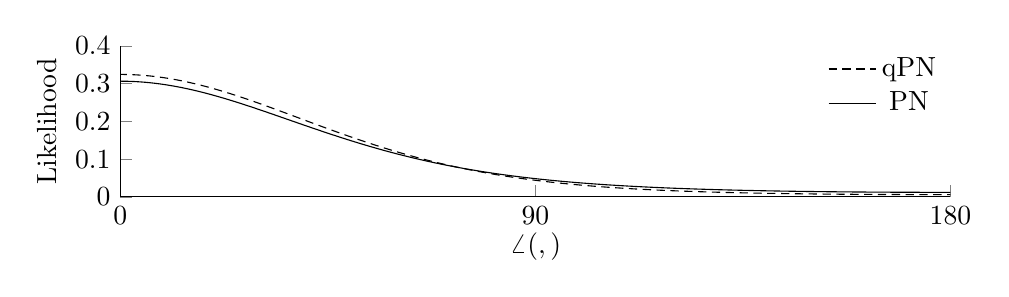
\begin{tikzpicture}
\begin{axis}[
width=\textwidth,
height=3.5cm,
%xmin=-180,
xmin=0,
xmax=180,
xtick={-180, -90, 0, 90, 180},
%xlabel={$\angle(\bbf, \bmu)$ (\textsuperscript{$\circ$})},
xlabel={$\angle(\bbf, \bmu) \vphantom{\rho}$},
xlabel shift=-4pt,
ymin=0,
ymax=0.4,
ytick={0, 0.1,0.2,0.3,0.4},
%ylabel={Relative Likelihood},
ylabel={Likelihood},
%ylabel shift = 1 pt
axis x line*=bottom,
axis y line*=left,
%ymajorticks=false,
%ylabel near ticks,
%hide y axis,
legend entries={qPN,PN},
legend style={draw=none, at={(1,1)}, anchor=north east},
%legend pos=north east,
]

%\addplot [only marks, mark size=2.5pt, mark=*, mark options={solid, black}]
%table[row sep=\\]{
%1 10\\
%};

% vMF for rho = 1
\addplot [black, densely dashed] table [row sep=newline]{
-180	0.00593882225388289
-179.099549774887	0.00594028921694383
-178.199099549775	0.00594469191800688
-177.298649324662	0.00595203579548720
-176.398199099550	0.00596232992266134
-175.497748874437	0.00597558702155373
-174.597298649325	0.00599182348239717
-173.696848424212	0.00601105938868620
-172.796398199100	0.00603331854784825
-171.895947973987	0.00605862852756205
-170.995497748874	0.00608702069775855
-170.095047523762	0.00611853027834409
-169.194597298649	0.00615319639269101
-168.294147073537	0.00619106212694495
-167.393696848424	0.00623217459520314
-166.493246623312	0.00627658501062192
-165.592796398199	0.00632434876251575
-164.692346173087	0.00637552549951384
-163.791895947974	0.00643017921884367
-162.891445722861	0.00648837836181406
-161.990995497749	0.00655019591557253
-161.090545272636	0.00661570952121452
-160.190095047524	0.00668500158832337
-159.289644822411	0.00675815941602121
-158.389194597299	0.00683527532061170
-157.488744372186	0.00691644676989561
-156.588294147074	0.00700177652423943
-155.687843921961	0.00709137278447597
-154.787393696848	0.00718534934671393
-153.886943471736	0.00728382576413018
-152.986493246623	0.00738692751581490
-152.086043021511	0.00749478618273469
-151.185592796398	0.00760753963087304
-150.285142571286	0.00772533220160043
-149.384692346173	0.00784831490931819
-148.484242121061	0.00797664564641068
-147.583791895948	0.00811048939552963
-146.683341670835	0.00825001844922190
-145.782891445723	0.00839541263689825
-144.882441220610	0.00854685955912501
-143.981990995498	0.00870455482920320
-143.081540770385	0.00886870232198060
-142.181090545273	0.00903951442982089
-141.280640320160	0.00921721232563079
-140.380190095048	0.00940202623282070
-139.479739869935	0.00959419570204657
-138.579289644822	0.00979396989455021
-137.678839419710	0.0100016078718829
-136.778389194597	0.0102173788917613
-135.877938969485	0.0104415627097664
-134.977488744372	0.0106744498865556
-134.077038519260	0.0109163421002126
-133.176588294147	0.0111675524633138
-132.276138069035	0.0114284058442382
-131.375687843922	0.0116992391921942
-130.475237618809	0.0119804018653788
-129.574787393697	0.0122722559616246
-128.674337168584	0.0125751766508230
-127.773886943472	0.0128895525083474
-126.873436718359	0.0132157858486230
-125.972986493247	0.0135542930579177
-125.072536268134	0.0139055049253465
-124.172086043022	0.0142698669709984
-123.271635817909	0.0146478397700064
-122.371185592796	0.0150398992712908
-121.470735367684	0.0154465371096080
-120.570285142571	0.0158682609094400
-119.669834917459	0.0163055945791553
-118.769384692346	0.0167590785937651
-117.868934467234	0.0172292702644899
-116.968484242121	0.0177167439932367
-116.068034017009	0.0182220915099724
-115.167583791896	0.0187459220908591
-114.267133566783	0.0192888627548955
-113.366683341671	0.0198515584366881
-112.466233116558	0.0204346721328465
-111.565782891446	0.0210388850193775
-110.665332666333	0.0216648965373200
-109.764882441221	0.0223134244437436
-108.864432216108	0.0229852048251019
-107.963981990996	0.0236809920698135
-107.063531765883	0.0244015587968176
-106.163081540770	0.0251476957367373
-105.262631315658	0.0259202115621660
-104.362181090545	0.0267199326634852
-103.461730865433	0.0275477028665194
-102.561280640320	0.0284043830882373
-101.660830415208	0.0292908509266224
-100.760380190095	0.0302080001807604
-99.8599299649825	0.0311567402971212
-98.9594797398700	0.0321379957379657
-98.0590295147574	0.0331527052677639
-97.1585792896448	0.0342018211534897
-96.2581290645323	0.0352863082746524
-95.3576788394197	0.0364071431389349
-94.4572286143072	0.0375653127993466
-93.5567783891946	0.0387618136688487
-92.6563281640820	0.0399976502284956
-91.7558779389695	0.0412738336252365
-90.8554277138569	0.0425913801556567
-89.9549774887444	0.0439513096320993
-89.0545272636318	0.0453546436278014
-88.1540770385193	0.0468024035979032
-87.2536268134067	0.0482956088734487
-86.3531765882942	0.0498352745257916
-85.4527263631816	0.0514224090991508
-84.5522761380690	0.0530580122094313
-83.6518259129565	0.0547430720078351
-82.7513756878439	0.0564785625082354
-81.8509254627314	0.0582654407777803
-80.9504752376188	0.0601046439907230
-80.0500250125063	0.0619970863460492
-79.1495747873937	0.0639436558500913
-78.2491245622811	0.0659452109659746
-77.3486743371686	0.0680025771324419
-76.4482241120560	0.0701165431553428
-75.5477738869435	0.0722878574758518
-74.6473236618309	0.0745172243202989
-73.7468734367184	0.0768052997373481
-72.8464232116058	0.0791526875291440
-71.9459729864932	0.0815599350839663
-71.0455227613807	0.0840275291188753
-70.1450725362682	0.0865558913417989
-69.2446223111556	0.0891453740434987
-68.3441720860430	0.0917962556308582
-67.4437218609305	0.0945087361139464
-66.5432716358179	0.0972829325603250
-65.6428214107053	0.100118874531089
-64.7423711855928	0.103016499514127
-63.8419209604802	0.105975648371097
-62.9414707353677	0.108996060815557
-62.0410205102551	0.112077370940665
-61.1405702851426	0.115219102815727
-60.2401200600300	0.118420666171763
-59.3396698349175	0.121681352197045
-58.4392196098049	0.125000329464289
-57.5387693846923	0.128376640011893
-56.6383191595798	0.131809195602141
-55.7378689344672	0.135296774179841
-54.8374187093547	0.138838016555232
-53.9369684842421	0.142431423335300
-53.0365182591296	0.146075352127816
-52.1360680340170	0.149768015042453
-51.2356178089045	0.153507476513277
-50.3351675837919	0.157291651466663
-49.4347173586793	0.161118303858358
-48.5342671335668	0.164985045602857
-47.6338169084542	0.168889335917619
-46.7333666833417	0.172828481103815
-45.8329164582291	0.176799634784276
-44.9324662331166	0.180799798618193
-44.0320160080040	0.184825823510745
-43.1315657828915	0.188874411334372
-42.2311155577789	0.192942117176725
-41.3306653326663	0.197025352128509
-40.4302151075538	0.201120386622447
-39.5297648824412	0.205223354332458
-38.6293146573287	0.209330256639849
-37.7288644322161	0.213436967670909
-36.8284142071036	0.217539239907724
-35.9279639819910	0.221632710371378
-35.0275137568784	0.225712907373920
-34.1270635317659	0.229775257832610
-33.2266133066533	0.233815095137021
-32.3261630815408	0.237827667556573
-31.4257128564282	0.241808147173025
-30.5252626313157	0.245751639319396
-29.6248124062031	0.249653192503717
-28.7243621810905	0.253507808792959
-27.8239119559780	0.257310454629482
-26.9234617308654	0.261056072049395
-26.0230115057529	0.264739590269345
-25.1225612806403	0.268355937605495
-24.2221110555278	0.271900053685817
-23.3216608304152	0.275366901914323
-22.4212106053026	0.278751482143549
-21.5207603801901	0.282048843509474
-20.6203101550775	0.285254097381142
-19.7198599299650	0.288362430375528
-18.8194097048524	0.291369117386807
-17.9189594797399	0.294269534577931
-17.0185092546273	0.297059172281551
-16.1180590295148	0.299733647756692
-15.2176088044022	0.302288717747257
-14.3171585792896	0.304720290788432
-13.4167083541771	0.307024439207360
-12.5162581290645	0.309197410765067
-11.6158079039520	0.311235639887556
-10.7153576788394	0.313135758435248
-9.81490745372686	0.314894605961522
-8.91445722861431	0.316509239412957
-8.01400700350175	0.317976942226093
-7.11355677838920	0.319295232777978
-6.21310655327664	0.320461872150507
-5.31265632816408	0.321474871171589
-4.41220610305153	0.322332496699389
-3.51175587793897	0.323033277119411
-2.61130565282641	0.323576007027809
-1.71085542771386	0.323959751078206
-0.810405202601301	0.324183846973289
0.0900450225112556	0.324247907586555
0.990495247623812	0.324151822203856
1.89094547273637	0.323895756878645
2.79139569784892	0.323480153899192
3.69184592296148	0.322905730370374
4.59229614807404	0.322173475916992
5.49274637318659	0.321284649519833
6.39319659829915	0.320240775499918
7.29364682341171	0.319043638670494
8.19409704852426	0.317695278680277
9.09454727363682	0.316197983575280
9.99499749874938	0.314554282610218
10.8954477238619	0.312766938343857
11.7958979489745	0.310838938055944
12.6963481740870	0.308773484526241
13.5967983991996	0.306573986218938
14.4972486243122	0.304244046918075
15.3976988494247	0.301787454861779
16.2981490745373	0.299208171424888
17.1985992996498	0.296510319401079
18.0990495247624	0.293698170936778
18.9994997498749	0.290776135170035
19.8999499749875	0.287748745628064
20.8004002001001	0.284620647437413
21.7008504252126	0.281396584400635
22.6013006503252	0.278081385992965
23.5017508754377	0.274679954331800
24.4022011005503	0.271197251170849
25.3026513256628	0.267638284969552
26.2031015507754	0.264008098086887
27.1035517758879	0.260311754146935
28.0040020010005	0.256554325621615
28.9044522261131	0.252740881673818
29.8049024512256	0.248876476301843
30.7053526763382	0.244966136823481
31.6058029014507	0.241014852735445
32.5062531265633	0.237027564981075
33.4067033516758	0.233009155656326
34.3071535767884	0.228964438181105
35.2076038019010	0.224898147960011
36.1080540270135	0.220814933553444
37.0085042521261	0.216719348377025
37.9089544772386	0.212615842944160
38.8094047023512	0.208508757663596
39.7098549274637	0.204402316200782
40.6103051525763	0.200300619408942
41.5107553776888	0.196207639832926
42.4112056028014	0.192127216786127
43.3116558279140	0.188063051998118
44.2121060530265	0.184018705828143
45.1125562781391	0.179997594037169
46.0130065032516	0.176002985108988
46.9134567283642	0.172037998108720
47.8139069534767	0.168105601065130
48.7143571785893	0.164208609861365
49.6148074037019	0.160349687617115
50.5152576288144	0.156531344543698
51.4157078539270	0.152755938252314
52.3161580790395	0.149025674494559
53.2166083041521	0.145342608313332
54.1170585292646	0.141708645581482
55.0175087543772	0.138125544904884
55.9179589794898	0.134594919866156
56.8184092046023	0.131118241584907
57.7188594297149	0.127696841570189
58.6193096548274	0.124331914840811
59.5197598799400	0.121024523289202
60.4202101050525	0.117775599264758
61.3206603301651	0.114585949352893
62.2211105552777	0.111456258326433
63.1215607803902	0.108387093246516
64.0220110055028	0.105378907690763
64.9224612306153	0.102432046087175
65.8229114557279	0.0995467481329287
66.7233616808404	0.0967231532781166
67.6238119059530	0.0939613052552814
68.5242621310655	0.0912611566365539
69.4247123561781	0.0886225734011217
70.3251625812906	0.0860453394967439
71.2256128064032	0.0835291613800178
72.1260630315158	0.0810736725211163
73.0265132566283	0.0786784378597283
73.9269634817409	0.0763429581999501
74.8274137068534	0.0740666745328909
75.7278639319660	0.0718489722767505
76.6283141570786	0.0696891854251139
77.5287643821911	0.0675866005951714
78.4292146073037	0.0655404609685113
79.3296648324162	0.0635499701180427
80.2301150575288	0.0616142957154864
81.1305652826413	0.0597325731147192
82.0310155077539	0.0579039088070629
82.9314657328664	0.0561273837453856
83.8319159579790	0.0544020565346108
84.7323661830915	0.0527269664869240
85.6328164082041	0.0511011365406147
86.5332666333167	0.0495235760421009
87.4337168584292	0.0479932833912480
88.3341670835418	0.0465092485506194
89.2346173086543	0.0450704554197764
90.1350675337669	0.0436758840761902
91.0355177588794	0.0423245128847245
91.9359679839920	0.0410153204780172
92.8364182091046	0.0397472876104059
93.7368684342171	0.0385193988883359
94.6373186593297	0.0373306443804387
95.5377688844422	0.0361800211106878
96.4382191095548	0.0350665344382275
97.3386693346673	0.0339891993276222
98.2391195597799	0.0329470415134061
99.1395697848924	0.0319390985629079
100.040020010005	0.0309644208414048
100.940470235118	0.0300220723837080
101.840920460230	0.0291111316763113
102.741370685343	0.0282306923542451
103.641820910455	0.0273798638167670
104.542271135568	0.0265577717659938
105.442721360680	0.0257635586725385
106.343171585793	0.0249963841721591
107.243621810905	0.0242554253973593
108.144072036018	0.0235398772478007
109.044522261131	0.0228489526032991
109.944972486243	0.0221818824830783
110.845422711356	0.0215379161548540
111.745872936468	0.0209163211972065
112.646323161581	0.0203163835185896
113.546773386693	0.0197374073362014
114.447223611806	0.0191787151178225
115.347673836918	0.0186396474896023
116.248124062031	0.0181195631126486
117.148574287144	0.0176178385311507
118.049024512256	0.0171338679946382
118.949474737369	0.0166670632568543
119.849924962481	0.0162168533535965
120.750375187594	0.0157826843617553
121.650825412706	0.0153640191416623
122.551275637819	0.0149603370647366
123.451725862931	0.0145711337283091
124.352176088044	0.0141959206593846
125.252626313157	0.0138342250089991
126.153076538269	0.0134855892387171
127.053526763382	0.0131495708007177
127.953976988494	0.0128257418128139
128.854427213607	0.0125136887296590
129.754877438719	0.0122130120113005
130.655327663832	0.0119233257901550
131.555777888944	0.0116442575373965
132.456228114057	0.0113754477296674
133.356678339170	0.0111165495169503
134.257128564282	0.0108672283923641
135.157578789395	0.0106271618645816
136.058029014507	0.0103960391335011
136.958479239620	0.0101735607697450
137.858929464732	0.00995943839850056
138.759379689845	0.00975339438816534
139.659829914958	0.00955516154420918
140.560280140070	0.00936448280861884
141.460730365183	0.00918111096524667
142.361180590295	0.00900480835134479
143.261630815408	0.00883534657552832
144.162081040520	0.00867250624237614
145.062531265633	0.00851607668384570
145.962981490745	0.00836585569764833
146.863431715858	0.00822164929270443
147.763881940971	0.00808327144177255
148.664332166083	0.00795054384132413
149.564782391196	0.00782329567871407
150.465232616308	0.00770136340667929
151.365682841421	0.00758459052517991
152.266133066533	0.00747282737058265
153.166583291646	0.00736593091217264
154.067033516758	0.00726376455596731
154.967483741871	0.00716619795579612
155.867933966984	0.00707310683159993
156.768384192096	0.00698437279489645
157.668834417209	0.00689988318135106
158.569284642321	0.00681953089038679
159.469734867434	0.00674321423176262
160.370185092546	0.00667083677904544
161.270635317659	0.00660230722989844
162.171085542771	0.00653753927310657
163.071535767884	0.00647645146225863
163.971985992996	0.00641896709600501
164.872436218109	0.00636501410481030
165.772886443222	0.00631452494412067
166.673336668334	0.00626743649386745
167.573786893447	0.00622368996423001
168.474237118559	0.00618323080758322
169.374687343672	0.00614600863655781
170.275137568784	0.00611197714814487
171.175587793897	0.00608109405377900
172.076038019010	0.00605332101533875
172.976488244122	0.00602862358700687
173.876938469235	0.00600697116293698
174.777388694347	0.00598833693067831
175.677838919460	0.00597269783031428
176.578289144572	0.00596003451927622
177.478739369685	0.00595033134279801
178.379189594797	0.00594357630998300
179.279639819910	0.00593976107545976
180	0.00593882225388289
};

%% PN
\addplot [black] table [row sep=newline]{
-180	0.0119906989306336
-179.099549774887	0.0119924933487507
-178.199099549775	0.0119978781223270
-177.298649324662	0.0120068578108691
-176.398199099550	0.0120194400196602
-175.497748874437	0.0120356354089268
-174.597298649325	0.0120554577066834
-173.696848424212	0.0120789237252725
-172.796398199100	0.0121060533816135
-171.895947973987	0.0121368697211852
-170.995497748874	0.0121713989457638
-170.095047523762	0.0122096704449472
-169.194597298649	0.0122517168314967
-168.294147073537	0.0122975739805326
-167.393696848424	0.0123472810726244
-166.493246623312	0.0124008806408154
-165.592796398199	0.0124584186216331
-164.692346173087	0.0125199444101309
-163.791895947974	0.0125855109190170
-162.891445722861	0.0126551746419258
-161.990995497749	0.0127289957208917
-161.090545272636	0.0128070380180870
-160.190095047524	0.0128893691918895
-159.289644822411	0.0129760607773467
-158.389194597299	0.0130671882711076
-157.488744372186	0.0131628312208932
-156.588294147074	0.0132630733195801
-155.687843921961	0.0133680025039734
-154.787393696848	0.0134777110583450
-153.886943471736	0.0135922957228169
-152.986493246623	0.0137118578066671
-152.086043021511	0.0138365033066380
-151.185592796398	0.0139663430303262
-150.285142571286	0.0141014927247333
-149.384692346173	0.0142420732100540
-148.484242121061	0.0143882105187790
-147.583791895948	0.0145400360401849
-146.683341670835	0.0146976866702847
-145.782891445723	0.0148613049673048
-144.882441220610	0.0150310393127519
-143.981990995498	0.0152070440781300
-143.081540770385	0.0153894797973578
-142.181090545273	0.0155785133449334
-141.280640320160	0.0157743181198836
-140.380190095048	0.0159770742355263
-139.479739869935	0.0161869687150638
-138.579289644822	0.0164041956930150
-137.678839419710	0.0166289566224783
-136.778389194597	0.0168614604882065
-135.877938969485	0.0171019240254559
-134.977488744372	0.0173505719445543
-134.077038519260	0.0176076371611163
-133.176588294147	0.0178733610318069
-132.276138069035	0.0181479935955373
-131.375687843922	0.0184317938199456
-130.475237618809	0.0187250298529901
-129.574787393697	0.0190279792794509
-128.674337168584	0.0193409293821035
-127.773886943472	0.0196641774072886
-126.873436718359	0.0199980308345694
-125.972986493247	0.0203428076501180
-125.072536268134	0.0206988366234338
-124.172086043022	0.0210664575869432
-123.271635817909	0.0214460217179814
-122.371185592796	0.0218378918225958
-121.470735367684	0.0222424426205569
-120.570285142571	0.0226600610308921
-119.669834917459	0.0230911464571939
-118.769384692346	0.0235361110718786
-117.868934467234	0.0239953800984951
-116.968484242121	0.0244693920911020
-116.068034017009	0.0249585992096429
-115.167583791896	0.0254634674901583
-114.267133566783	0.0259844771085773
-113.366683341671	0.0265221226367289
-112.466233116558	0.0270769132891049
-111.565782891446	0.0276493731587966
-110.665332666333	0.0282400414409081
-109.764882441221	0.0288494726416270
-108.864432216108	0.0294782367710057
-107.963981990996	0.0301269195173747
-107.063531765883	0.0307961224011693
-106.163081540770	0.0314864629058132
-105.262631315658	0.0321985745831513
-104.362181090545	0.0329331071307785
-103.461730865433	0.0336907264384522
-102.561280640320	0.0344721146006246
-101.660830415208	0.0352779698919657
-100.760380190095	0.0361090067025907
-99.8599299649825	0.0369659554295389
-98.9594797398700	0.0378495623208916
-98.0590295147574	0.0387605892687499
-97.1585792896448	0.0396998135471348
-96.2581290645323	0.0406680274907127
-95.3576788394197	0.0416660381100942
-94.4572286143072	0.0426946666393070
-93.5567783891946	0.0437547480108987
-92.6563281640820	0.0448471302539957
-91.7558779389695	0.0459726738105186
-90.8554277138569	0.0471322507646448
-89.9549774887444	0.0483267439805150
-89.0545272636318	0.0495570461430989
-88.1540770385193	0.0508240586970770
-87.2536268134067	0.0521286906785591
-86.3531765882942	0.0534718574344416
-85.4527263631816	0.0548544792242272
-84.5522761380690	0.0562774796991667
-83.6518259129565	0.0577417842536665
-82.7513756878439	0.0592483182440138
-81.8509254627314	0.0607980050696284
-80.9504752376188	0.0623917641122447
-80.0500250125063	0.0640305085286670
-79.1495747873937	0.0657151428930373
-78.2491245622811	0.0674465606848951
-77.3486743371686	0.0692256416197082
-76.4482241120560	0.0710532488190156
-75.5477738869435	0.0729302258178402
-74.6473236618309	0.0748573934076153
-73.7468734367184	0.0768355463135238
-72.8464232116058	0.0788654497058654
-71.9459729864932	0.0809478355458653
-71.0455227613807	0.0830833987672009
-70.1450725362682	0.0852727932954634
-69.2446223111556	0.0875166279087852
-68.3441720860430	0.0898154619439534
-67.4437218609305	0.0921698008534908
-66.5432716358179	0.0945800916204203
-65.6428214107053	0.0970467180387348
-64.7423711855928	0.0995699958689617
-63.8419209604802	0.102150167879651
-62.9414707353677	0.104787398787101
-62.0410205102551	0.107481770107189
-61.1405702851426	0.110233274934753
-60.2401200600300	0.113041812667600
-59.3396698349175	0.115907183693877
-58.4392196098049	0.118829084063194
-57.5387693846923	0.121807100163588
-56.6383191595798	0.124840703428048
-55.7378689344672	0.127929245096019
-54.8374187093547	0.131071951056859
-53.9369684842421	0.134267916803817
-53.0365182591296	0.137516102528583
-52.1360680340170	0.140815328387842
-51.2356178089045	0.144164269974586
-50.3351675837919	0.147561454028085
-49.4347173586793	0.151005254417467
-48.5342671335668	0.154493888434676
-47.6338169084542	0.158025413433309
-46.7333666833417	0.161597723850231
-45.8329164582291	0.165208548647185
-44.9324662331166	0.168855449209545
-44.0320160080040	0.172535817739138
-43.1315657828915	0.176246876177505
-42.2311155577789	0.179985675695130
-41.3306653326663	0.183749096781007
-40.4302151075538	0.187533849965474
-39.5297648824412	0.191336477207404
-38.6293146573287	0.195153353974725
-37.7288644322161	0.198980692044767
-36.8284142071036	0.202814543048072
-35.9279639819910	0.206650802776185
-35.0275137568784	0.210485216270395
-34.1270635317659	0.214313383704607
-33.2266133066533	0.218130767071368
-32.3261630815408	0.221932697675633
-31.4257128564282	0.225714384436182
-30.5252626313157	0.229470922989612
-29.6248124062031	0.233197305586701
-28.7243621810905	0.236888431765564
-27.8239119559780	0.240539119780551
-26.9234617308654	0.244144118760249
-26.0230115057529	0.247698121562262
-25.1225612806403	0.251195778286845
-24.2221110555278	0.254631710405784
-23.3216608304152	0.258000525457425
-22.4212106053026	0.261296832253363
-21.5207603801901	0.264515256537099
-20.6203101550775	0.267650457030071
-19.7198599299650	0.270697141795823
-18.8194097048524	0.273650084848816
-17.9189594797399	0.276504142930569
-17.0185092546273	0.279254272372396
-16.1180590295148	0.281895545961159
-15.2176088044022	0.284423169722143
-14.3171585792896	0.286832499531416
-13.4167083541771	0.289119057468932
-12.5162581290645	0.291278547823218
-11.6158079039520	0.293306872658652
-10.7153576788394	0.295200146857297
-9.81490745372686	0.296954712548851
-8.91445722861431	0.298567152844551
-8.01400700350175	0.300034304793906
-7.11355677838920	0.301353271486775
-6.21310655327664	0.302521433227634
-5.31265632816408	0.303536457713867
-4.41220610305153	0.304396309155400
-3.51175587793897	0.305099256279153
-2.61130565282641	0.305643879168329
-1.71085542771386	0.306029074893636
-0.810405202601301	0.306254061900917
0.0900450225112556	0.306318383127454
0.990495247623812	0.306221907827150
1.89094547273637	0.305964832093011
2.79139569784892	0.305547678073595
3.69184592296148	0.304971291888406
4.59229614807404	0.304236840255493
5.49274637318659	0.303345805852625
6.39319659829915	0.302299981441372
7.29364682341171	0.301101462791123
8.19409704852426	0.299752640447376
9.09454727363682	0.298256190395652
9.99499749874938	0.296615063678810
10.8954477238619	0.294832475031592
11.7958979489745	0.292911890601618
12.6963481740870	0.290857014830893
13.5967983991996	0.288671776576093
14.4972486243122	0.286360314549431
15.3976988494247	0.283926962164750
16.2981490745373	0.281376231875679
17.1985992996498	0.278712799094137
18.0990495247624	0.275941485778241
18.9994997498749	0.273067243778772
19.8999499749875	0.270095138032765
20.8004002001001	0.267030329691546
21.7008504252126	0.263878059268716
22.6013006503252	0.260643629891121
23.5017508754377	0.257332390732894
24.4022011005503	0.253949720709172
25.3026513256628	0.250501012502138
26.2031015507754	0.246991656987747
27.1035517758879	0.243427028126757
28.0040020010005	0.239812468378738
28.9044522261131	0.236153274692489
29.8049024512256	0.232454685120866
30.7053526763382	0.228721866102504
31.6058029014507	0.224959900447232
32.5062531265633	0.221173776056372
33.4067033516758	0.217368375403432
34.3071535767884	0.213548465795149
35.2076038019010	0.209718690427359
36.1080540270135	0.205883560244867
37.0085042521261	0.202047446609377
37.9089544772386	0.198214574774610
38.8094047023512	0.194389018163117
39.7098549274637	0.190574693434904
40.6103051525763	0.186775356333922
41.5107553776888	0.182994598294684
42.4112056028014	0.179235843787884
43.3116558279140	0.175502348380736
44.2121060530265	0.171797197485050
45.1125562781391	0.168123305763601
46.0130065032516	0.164483417163314
46.9134567283642	0.160880105542022
47.8139069534767	0.157315775854166
48.7143571785893	0.153792665859714
49.6148074037019	0.150312848319809
50.5152576288144	0.146878233642130
51.4157078539270	0.143490572938805
52.3161580790395	0.140151461459694
53.2166083041521	0.136862342364202
54.1170585292646	0.133624510795262
55.0175087543772	0.130439118219859
55.9179589794898	0.127307177001348
56.8184092046023	0.124229565169881
57.7188594297149	0.121207031358439
58.6193096548274	0.118240199873322
59.5197598799400	0.115329575869312
60.4202101050525	0.112475550601280
61.3206603301651	0.109678406725546
62.2211105552777	0.106938323625934
63.1215607803902	0.104255382741110
64.0220110055028	0.101629572871462
64.9224612306153	0.0990607954454620
65.8229114557279	0.0965488697271070
66.7233616808404	0.0940935379476967
67.6238119059530	0.0916944703468125
68.5242621310655	0.0893512701089511
69.4247123561781	0.0870634781837980
70.3251625812906	0.0848305779796060
71.2256128064032	0.0826519999205657
72.1260630315158	0.0805271258604151
73.0265132566283	0.0784552933458236
73.9269634817409	0.0764357997243074
74.8274137068534	0.0744679060925798
75.7278639319660	0.0725508410823142
76.6283141570786	0.0706838044812976
77.5287643821911	0.0688659706888748
78.4292146073037	0.0670964920054378
79.3296648324162	0.0653745017564913
80.2301150575288	0.0636991172525342
81.1305652826413	0.0620694425866342
82.0310155077539	0.0604845712721466
82.9314657328664	0.0589435887235342
83.8319159579790	0.0574455745836922
84.7323661830915	0.0559896049015723
85.6328164082041	0.0545747541642304
86.5332666333167	0.0532000971877051
87.4337168584292	0.0518647108713675
88.3341670835418	0.0505676758205666
89.2346173086543	0.0493080778425443
90.1350675337669	0.0480850093206959
91.0355177588794	0.0468975704723242
91.9359679839920	0.0457448704950738
92.8364182091046	0.0446260286072388
93.7368684342171	0.0435401749871184
94.6373186593297	0.0424864516165557
95.5377688844422	0.0414640130337261
96.4382191095548	0.0404720270001645
97.3386693346673	0.0395096750869173
98.2391195597799	0.0385761531845954
99.1395697848924	0.0376706719419775
100.040020010005	0.0367924571376785
100.940470235118	0.0359407499892537
101.840920460230	0.0351148074039608
102.741370685343	0.0343139021752434
103.641820910455	0.0335373231288448
104.542271135568	0.0327843752222949
105.442721360680	0.0320543796013528
106.343171585793	0.0313466736168243
107.243621810905	0.0306606108050087
108.144072036018	0.0299955608348703
109.044522261131	0.0293509094248696
109.944972486243	0.0287260582322320
110.845422711356	0.0281204247172808
111.745872936468	0.0275334419853084
112.646323161581	0.0269645586083166
113.546773386693	0.0264132384288159
114.447223611806	0.0258789603477341
115.347673836918	0.0253612180983568
116.248124062031	0.0248595200080942
117.148574287144	0.0243733887497451
118.049024512256	0.0239023610838160
118.949474737369	0.0234459875933402
119.849924962481	0.0230038324125352
120.750375187594	0.0225754729505372
121.650825412706	0.0221604996113556
122.551275637819	0.0217585155110976
123.451725862931	0.0213691361934304
124.352176088044	0.0209919893441646
125.252626313157	0.0206267145057666
126.153076538269	0.0202729627925378
127.053526763382	0.0199303966071268
127.953976988494	0.0195986893589825
128.854427213607	0.0192775251852916
129.754877438719	0.0189665986748924
130.655327663832	0.0186656145956038
131.555777888944	0.0183742876253586
132.456228114057	0.0180923420874891
133.356678339170	0.0178195116904673
134.257128564282	0.0175555392723672
135.157578789395	0.0173001765502783
136.058029014507	0.0170531838748695
136.958479239620	0.0168143299902687
137.858929464732	0.0165833917994001
138.759379689845	0.0163601541348916
139.659829914958	0.0161444095356449
140.560280140070	0.0159359580291380
141.460730365183	0.0157346069195101
142.361180590295	0.0155401705814634
143.261630815408	0.0153524702599989
144.162081040520	0.0151713338759902
145.062531265633	0.0149965958375855
145.962981490745	0.0148280968574177
146.863431715858	0.0146656837755925
147.763881940971	0.0145092093884149
148.664332166083	0.0143585322828070
149.564782391196	0.0142135166763634
150.465232616308	0.0140740322629848
151.365682841421	0.0139399540640257
152.266133066533	0.0138111622848871
153.166583291646	0.0136875421769826
154.067033516758	0.0135689839050041
154.967483741871	0.0134553824194098
155.867933966984	0.0133466373340562
156.768384192096	0.0132426528088973
157.668834417209	0.0131433374376688
158.569284642321	0.0130486041404809
159.469734867434	0.0129583700612387
160.370185092546	0.0128725564698137
161.270635317659	0.0127910886688885
162.171085542771	0.0127138959054001
163.071535767884	0.0126409112865073
163.971985992996	0.0125720717000112
164.872436218109	0.0125073177391591
165.772886443222	0.0124465936317643
166.673336668334	0.0123898471735780
167.573786893447	0.0123370296658506
168.474237118559	0.0122880958570252
169.374687343672	0.0122430038885056
170.275137568784	0.0122017152444478
171.175587793897	0.0121641947055252
172.076038019010	0.0121304103066208
172.976488244122	0.0121003332984059
173.876938469235	0.0120739381127641
174.777388694347	0.0120512023320271
175.677838919460	0.0120321066619893
176.578289144572	0.0120166349086751
177.478739369685	0.0120047739588320
178.379189594797	0.0119965137641322
179.279639819910	0.0119918473290633
180	0.0119906989306336
};

\end{axis}
\end{tikzpicture}
        \vspace{-18pt}
        \caption{Relative likelihood ($\rho = 1$)}
        \label{fig:sub_label_c}
    \end{subfigure}\hfill % any excess horizontal space goes between the subfigures
    \begin{subfigure}[]{0.33\linewidth}\centering
        \begin{tikzpicture}
\begin{axis}[
scaled ticks=false,
tick label style={/pgf/number format/fixed},
width=\textwidth,
height=3.5cm,
xmin=0,
xmax=5,
xtick={0, 1, ..., 5},
xlabel={$\rho \vphantom{\angle(\bbf, \bmu)}$},
xlabel shift=-4pt,
ymin=0,
ymax=0.04,
ytick={0, 0.01, ...,0.04},
ylabel={MAE},
%ylabel shift=-2pt,
axis x line*=bottom,
axis y line*=left,
%ymajorticks=false,
%ylabel near ticks,
%hide y axis,
%legend entries={$\vMF$,$\PN$},
%legend style={draw=none, at={(1,1)}, anchor=north east},
%legend pos=north east,
]

%\addplot [only marks, mark size=2.5pt, mark=*, mark options={solid, black}]
%table[row sep=\\]{
%1 10\\
%};

%% MAE
\addplot [black] table [row sep=newline]{
0.100000000000000	0.0413191281236007
0.200000000000000	0.0346139984696496
0.300000000000000	0.0287655282865310
0.400000000000000	0.0237540068813730
0.500000000000000	0.0195422603081568
0.600000000000000	0.0160829910864740
0.700000000000000	0.0133195988920811
0.800000000000000	0.0111819311945709
0.900000000000000	0.00959030244918633
1	0.00845004251628531
1.10000000000000	0.00766221054548387
1.20000000000000	0.00713263091784733
1.30000000000000	0.00678074719239092
1.40000000000000	0.00654514421515479
1.50000000000000	0.00637890241051719
1.60000000000000	0.00625222568688656
1.70000000000000	0.00614385236628324
1.80000000000000	0.00604225040266751
1.90000000000000	0.00594325703404724
2	0.00584243421372227
2.10000000000000	0.00573946498348980
2.20000000000000	0.00563494957933974
2.30000000000000	0.00552965882016238
2.40000000000000	0.00542408740054571
2.50000000000000	0.00531819228966805
2.60000000000000	0.00521173034184175
2.70000000000000	0.00510893640257420
2.80000000000000	0.00500440880697224
2.90000000000000	0.00490423025006244
3.00000000000000	0.00480464961892366
3.10000000000000	0.00470596094922317
3.20000000000000	0.00460899176414898
3.30000000000000	0.00451506785319796
3.40000000000000	0.00442358842394028
3.50000000000000	0.00433382063316873
3.60000000000000	0.00424710238945909
3.70000000000000	0.00416346872314328
3.80000000000000	0.00408199500296547
3.90000000000000	0.00400204393072496
4	0.00392277575732362
4.10000000000000	0.00384711043735623
4.20000000000000	0.00377563566639987
4.30000000000000	0.00370306328274511
4.40000000000000	0.00363438691018970
4.50000000000000	0.00356863657853114
4.60000000000000	0.00350096684493657
4.70000000000000	0.00344123882469621
4.80000000000000	0.00337624008011355
4.90000000000000	0.00332126663698587
5.00000000000000	0.00326021275980349
5.10000000000000	0.00320831280363775
5.20000000000000	0.00315218952938847
5.30000000000000	0.00310128823298805
5.40000000000000	0.00305087424444898
5.50000000000000	0.00299849472816950
5.60000000000000	0.00295442142273135
5.70000000000000	0.00290599225929935
5.80000000000000	0.00286044892770108
5.90000000000000	0.00281913064321619
6	0.00277412406175830
6.10000000000000	0.00273221253592677
6.20000000000000	0.00269484671225199
6.30000000000000	0.00265427356087413
6.40000000000000	0.00261227041931178
6.50000000000000	0.00257972468941359
6.60000000000000	0.00254431821113954
6.70000000000000	0.00250632851637804
6.80000000000000	0.00247084860356331
6.90000000000000	0.00244116499294787
7	0.00240910028589179
7.10000000000000	0.00237487578991004
7.20000000000000	0.00234078460131801
7.30000000000000	0.00231503276864338
7.40000000000000	0.00228723026026129
7.50000000000000	0.00225755230706364
7.60000000000000	0.00222617117499046
7.70000000000000	0.00219797456116073
7.80000000000000	0.00217507443548226
7.90000000000000	0.00215049223483861
8	0.00212436344258786
8.10000000000000	0.00209682136295644
8.20000000000000	0.00206799676653635
8.30000000000000	0.00204845650327287
8.40000000000000	0.00202794580224906
8.50000000000000	0.00200610148667098
8.60000000000000	0.00198302589451114
8.70000000000000	0.00195881974468721
8.80000000000000	0.00193358190998049
8.90000000000000	0.00191431249473836
9	0.00189725321466546
9.10000000000000	0.00187908073990816
9.20000000000000	0.00185987160506170
9.30000000000000	0.00183970132685681
9.40000000000000	0.00181864425438302
9.50000000000000	0.00179677342856303
9.60000000000000	0.00177741929741420
9.70000000000000	0.00176350894505390
9.80000000000000	0.00174868562616075
9.90000000000000	0.00173300508406668
10	0.00171652245632889
};

\end{axis}
\end{tikzpicture}
        \vspace{-18pt}
        \caption{Mean Absolute Error}
        \label{fig:sub_label_d}
    \end{subfigure}\hfill
    \begin{subfigure}[]{0.33\linewidth}\centering
        \begin{tikzpicture}
\begin{axis}[
scaled ticks=false,
tick label style={/pgf/number format/fixed},
width=\textwidth,
height=3.5cm,
xmin=0,
xmax=5,
xtick={0, 1, ..., 5},
xlabel={$\rho \vphantom{\angle(\bbf, \bmu)}$},
xlabel shift=-4pt,
ymin=0,
ymax=0.04,
ytick={0, 0.01, ...,0.04},
ylabel={MAE},
%ylabel shift=-2pt,
axis x line*=bottom,
axis y line*=left,
%ymajorticks=false,
%ylabel near ticks,
%hide y axis,
%legend entries={$\vMF$,$\PN$},
%legend style={draw=none, at={(1,1)}, anchor=north east},
%legend pos=north east,
]

%\addplot [only marks, mark size=2.5pt, mark=*, mark options={solid, black}]
%table[row sep=\\]{
%1 10\\
%};

%% MAE
\addplot [black] table [row sep=newline]{
0.100000000000000	0.0413191281236007
0.200000000000000	0.0346139984696496
0.300000000000000	0.0287655282865310
0.400000000000000	0.0237540068813730
0.500000000000000	0.0195422603081568
0.600000000000000	0.0160829910864740
0.700000000000000	0.0133195988920811
0.800000000000000	0.0111819311945709
0.900000000000000	0.00959030244918633
1	0.00845004251628531
1.10000000000000	0.00766221054548387
1.20000000000000	0.00713263091784733
1.30000000000000	0.00678074719239092
1.40000000000000	0.00654514421515479
1.50000000000000	0.00637890241051719
1.60000000000000	0.00625222568688656
1.70000000000000	0.00614385236628324
1.80000000000000	0.00604225040266751
1.90000000000000	0.00594325703404724
2	0.00584243421372227
2.10000000000000	0.00573946498348980
2.20000000000000	0.00563494957933974
2.30000000000000	0.00552965882016238
2.40000000000000	0.00542408740054571
2.50000000000000	0.00531819228966805
2.60000000000000	0.00521173034184175
2.70000000000000	0.00510893640257420
2.80000000000000	0.00500440880697224
2.90000000000000	0.00490423025006244
3.00000000000000	0.00480464961892366
3.10000000000000	0.00470596094922317
3.20000000000000	0.00460899176414898
3.30000000000000	0.00451506785319796
3.40000000000000	0.00442358842394028
3.50000000000000	0.00433382063316873
3.60000000000000	0.00424710238945909
3.70000000000000	0.00416346872314328
3.80000000000000	0.00408199500296547
3.90000000000000	0.00400204393072496
4	0.00392277575732362
4.10000000000000	0.00384711043735623
4.20000000000000	0.00377563566639987
4.30000000000000	0.00370306328274511
4.40000000000000	0.00363438691018970
4.50000000000000	0.00356863657853114
4.60000000000000	0.00350096684493657
4.70000000000000	0.00344123882469621
4.80000000000000	0.00337624008011355
4.90000000000000	0.00332126663698587
5.00000000000000	0.00326021275980349
5.10000000000000	0.00320831280363775
5.20000000000000	0.00315218952938847
5.30000000000000	0.00310128823298805
5.40000000000000	0.00305087424444898
5.50000000000000	0.00299849472816950
5.60000000000000	0.00295442142273135
5.70000000000000	0.00290599225929935
5.80000000000000	0.00286044892770108
5.90000000000000	0.00281913064321619
6	0.00277412406175830
6.10000000000000	0.00273221253592677
6.20000000000000	0.00269484671225199
6.30000000000000	0.00265427356087413
6.40000000000000	0.00261227041931178
6.50000000000000	0.00257972468941359
6.60000000000000	0.00254431821113954
6.70000000000000	0.00250632851637804
6.80000000000000	0.00247084860356331
6.90000000000000	0.00244116499294787
7	0.00240910028589179
7.10000000000000	0.00237487578991004
7.20000000000000	0.00234078460131801
7.30000000000000	0.00231503276864338
7.40000000000000	0.00228723026026129
7.50000000000000	0.00225755230706364
7.60000000000000	0.00222617117499046
7.70000000000000	0.00219797456116073
7.80000000000000	0.00217507443548226
7.90000000000000	0.00215049223483861
8	0.00212436344258786
8.10000000000000	0.00209682136295644
8.20000000000000	0.00206799676653635
8.30000000000000	0.00204845650327287
8.40000000000000	0.00202794580224906
8.50000000000000	0.00200610148667098
8.60000000000000	0.00198302589451114
8.70000000000000	0.00195881974468721
8.80000000000000	0.00193358190998049
8.90000000000000	0.00191431249473836
9	0.00189725321466546
9.10000000000000	0.00187908073990816
9.20000000000000	0.00185987160506170
9.30000000000000	0.00183970132685681
9.40000000000000	0.00181864425438302
9.50000000000000	0.00179677342856303
9.60000000000000	0.00177741929741420
9.70000000000000	0.00176350894505390
9.80000000000000	0.00174868562616075
9.90000000000000	0.00173300508406668
10	0.00171652245632889
};

\end{axis}
\end{tikzpicture}
        \vspace{-18pt}
        \caption{Mean Absolute Error}
        \label{fig:sub_label_e}
    \end{subfigure}%
    \caption{Main caption here. \subref{fig:sub_label_a} A nice plot in Tikz. \subref{fig:sub_label_b} Also something. \subref{fig:sub_label_c} Ground truth. \subref{fig:sub_label_d} ???? \subref{fig:sub_label_e} !!!!}
    \label{fig:subfig}
\end{figure}

% tikz: high quality vector graphics (diagrams) including in 3D; pgfplots: graphs and data management

% Mathematics:
Inline symbols like this $\Gamma = 0.01$. The flow rate is given by
\begin{equation}
    r = 2VP,
    \label{eq:flowrate}
\end{equation}
where the volume is denoted by $V$ and blah. As shown in \Cref{eq:flowrate}, we see\dots
The other equation environment is this one
\begin{align}
    E &= mc^2\\
      &= m(1-p)\\
      &\rightarrow \sum_{i=1}^{N} w_i \hat{x},
\end{align}
where\dots
$\bv \in \reals^n$ and the loss $\cL_\text{heatmap}$.
Can declare math operators in the macros.
\begin{equation}
    x =
    \begin{cases}
        1 \text{ if bingo,}\\
        2 \text{ otherwise.}
    \end{cases}
\end{equation}

% Referencing:
% Sentence should make sense if you delete the parts inside the parentheses
% Google Scholar
% Use official details rather than arxiv version where possible
% @inproceedings for conferences
% @article for journal articles
% @misc for websites
% ANU library has details on how to do these
For example, these people \citep{engelhardt2024shinobi,Cooper2015SuperfluidVacuumTheory,Oetiker2021LatexIntroduction}.
\citet{Cooper2015SuperfluidVacuumTheory} believe\dots
The trial is stacked \citep{Cooper2015SuperfluidVacuumTheory}.

% References (non-bibliographic):
\Cref{chap:background}
\Cref{eq:flowrate}
\Cref{fig:pageBorders}

% Lists:
\begin{enumerate}
    \item ordered elements
    \item like this
\end{enumerate}
\begin{itemize}
    \item unordered elements
    \item like this
\end{itemize}

% Misc:
% Formal language: no contractions, no idioms
% Clear communication is the goal: precise, concrete examples, reference everything
% First person or passive
% spell-check
% no random capitalisation, only proper nouns or at sentence start
% do not over-use bold or italics
% macros: see macro.tex -- define your own and use them
Smith \etal believe X \citep{Smith2021Wubalubadubdub}.
Jelly, \eg, aeroplane, is good.
Jelly, \ie, aeroplane, is good.
% quotation marks
``Quote here''. % note the ``
% -,--,---
Compound words get hyphens like self-attention. Those hard-to-reach locations.
En dashes are used for ranges like 2--5, and if you have two complete words that you are joining, like Navier--Stokes Theorem or 2D--3D projection.
Em dashes are for emphatic subclauses---like this one---in the middle of a sentence.

% Advice:
%% How to start? Write down all section titles, then subsections, then add a few dot points about what you want to say in each, then fill them out
%% Put in placeholder (empty) figures and tables with a note in the caption saying what you want to be there.
%% Use latex comments (like this) to structure your thoughts. E.g.,

% Task:
This thesis considers the task of\dots
%
% Motivation:
This is a key component of many driver safety systems and so any efficiency improvements have real-world implications.
% Challenges:
However, it's a pain.

This chapter holds your contributions. Depending on your exact topic, you might use only a single chapter for your actual contributions, or several. Even having several is not unusual. Discuss your proposal with your supervisor(s) and propose descriptive titles. 

The following sections give additional advice that is specifically tailored to students who are new to either \LaTeX{} or scientific writing. I \emph{strongly} suggest that you read the entire document carefully! Also use it as checklist after you started writing and after finishing.


\section{Abstract Advice}

\begin{itemize}
 \item \textbf{Start early.} Writing a report is hard and takes time. More than you think. \emph{Hofstadter's Law:} ``It always takes longer than you expect, even when you take into account Hofstadter's Law.'' -- \emph{So start early!}
 \item \textbf{Read and check your work!} Each \LaTeX{} editor has a spellchecker. Use it!! Read your work \emph{carefully} and \emph{multiple times} before showing it to your supervisor. And \emph{please} read the next sections before doing so! I \emph{guarantee} that it explains errors that you do! Prevent them! Use the next section as checklist!
 \item \textbf{Involve your supervisor!} Don't be afraid to reach out to your supervisor(s)! It's quite literally his/her/their job to supervise you and help you succeed! :) So make sure you get what you need to be successful, don't hold back. But make it easy for them. Most academics are overworked...
 \item \textbf{Choose your title page.} This template has two distinct title pages. Choose the one you like more by setting up the configuration file accordingly. You could even change the template if you like. It's not to restrict you but to save you time.

\end{itemize}

